\cleardoublepage

\chapter{Propuesta}
\label{ch:Capitulo3}

Se consideran 2 perfiles de usuarios que hacen uso de la solución domótica que creara. Por un lado, un  perfil de \verb|usuario| sin conocimientos específicos de informática. Su necesidad de domótica se centra en monitorizar aspectos ambientales del hogar, o manipular mediante un móvil las luces, pudiendo verificar si las luces están encendidas en una sala sin necesidad de ir a la misma. El segundo perfil, el de \verb|administrador| posee conocimientos de programación en lenguajes de alto y bajo nivel y gestión de un \gls{so} Linux. Sera el encargado de planificar, desplegar y gestionar la suite domótica en base a las especificaciones impuestas por el usuario.

\vspace{1cm}

Ambos perfiles han acordado que el coste de la solución domótica que se aplique, no debe exceder un presupuesto por encima de 100 euros en componentes. Esta restricción además, debe considerar que la escalabilidad de la solución tiene un alcance indefinido, pudiendo solicitarse la agregación a la red domótica de cualquier clase de sensor y actuador en el futuro. Sí esta definida sin embargo, la intención del usuario de monitorizar la temperatura de una estancia y su control de luces. Se obvian los costes de desarrollo, ya que en este supuesto escenario, el administrador ya ha decidido la creación de un despliegue de \gls{iot} propio, el cual esta reflejado en esta documentación. La estancia en la que se desarrolla el escenario es una habitación subterránea con un único acceso y sin ventanas. Dispone de múltiples puntos de conexión a la red eléctrica. El principal problema del usuario en la sala, es el interruptor de luz que no se encuentra junto a la puerta de entrada, si no bajando las escaleras. También preocupa la temperatura y humedad de la estancia en la cual se encuentran dos cubas caseras para fermentar vino. Si la temperatura no es estable, esto afectara a la calidad final del vino. Pero antes de determinar si en necesario instalar equitaciones deshumidificadoras, o sistemas de climatización, hay que conocer la situación actual. El administrador expone el despliegue \gls{iot} que se aplicara en la estancia mostrado en la figura~\ref{scenary_proposal}.

\vspace{0.5cm}
\begin{figure}[hbt!]
\label{scenary_proposal}
\centering
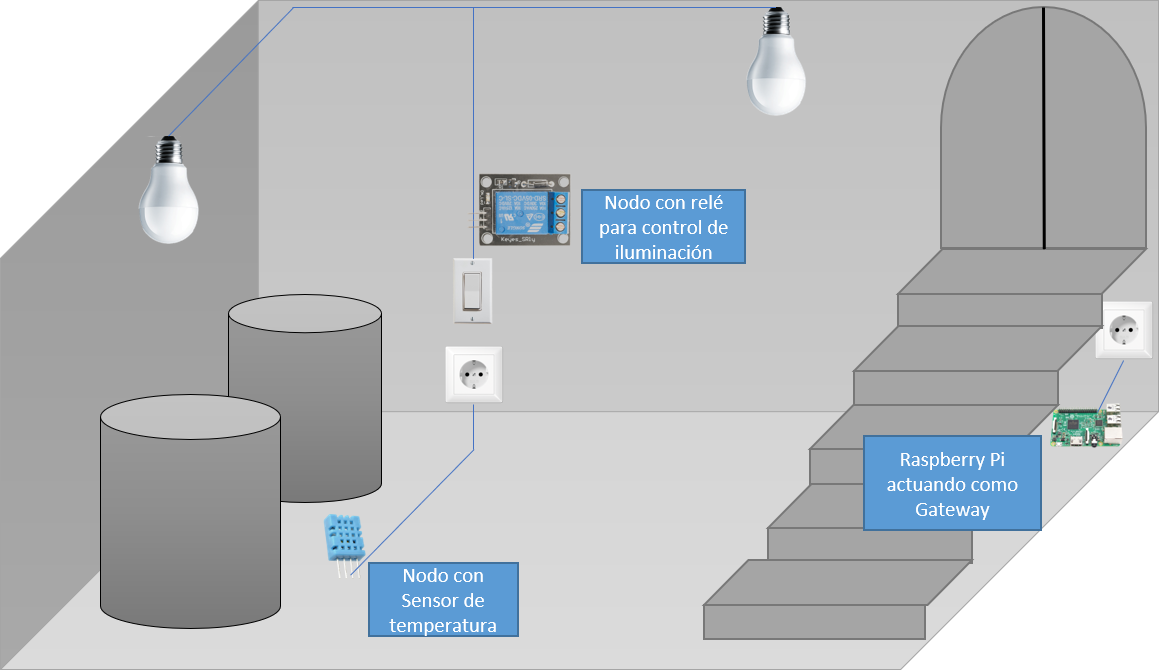
\includegraphics[height=3.5in]{figures/escenario_propuesto_comentado.png}
\caption[Escenario propuesto para el despliegue en una estancia]{Escenario propuesto para el despliegue en una estancia}
\end{figure}

\vspace{1cm}

Para facilitar el uso por parte del usuario de esta solución domótica, se instalar en su móvil una aplicación que permitirá gestionar la configuración del sistema, consultando los registros de los nodos sensores, los estados de los nodos actuadores, manipular dichos estados, y agregar nuevos nodos en el despliegue de una instancia, o generando instancias separadas para organizar con mas facilidad. Todo este abanico de casos de uso serán explicados en el capitulo~\ref{ch:Capitulo5}. Para flexibilizar su uso a distancia es necesario que la aplicación gestione los dispositivos tanto desde dentro de la casa, como desde fuera. Eso implica que el administrador configure una redirección en el router domestico del hogar hacia un servidor ejecutado en un ordenador de la casa.

\vspace{1cm}

Aunque inicialmente el prototipo de solución domótica puede registrar temperaturas y humedad de una instancia así como alterar el estado de un relé, sera necesario planificar un método que permita al administrador agregar nuevos tipos de sensores y actuadores a las opciones disponibles. Eso implica crear programaciones especificas para cada tipo de dispositivo, y también la posibilidad de que cada nodo pueda ejecutarse sobre diferentes placas microcontroladoras, en función de las necesidad que puedan surgir.


\vspace{1cm}

La suite domótica sera ejecutada en un ordenador de bajo coste con capacidad inalámbrica, que permite la conexión de nodos inalámbricos con roles de actuador o sensor. Puede operar desde dentro de la red local en la que operan los nodos, o desde fuera de la misma con conexiones remotas, mediante una aplicación para dispositivo móvil con sistema operativo Android. Si bien, la operatividad remota es opcional, se debe alcanzar la gestión de la suite en el entorno de la red local, cumpliendo así con el objetivo de disponer de un sistema aislado y autónomo, que no dependa de servicios externos para su funcionamiento. Una vez alcanzada una implementación funcional del prototipo se aplicará en dos casos de usos que ejemplifican la entrada y salidas características de todo sistema de domótica, la recepción, proceso y presentación de datos de un dispositivo sensor en la aplicación móvil, y la gestión de un actuador desde dicha aplicación. Esta suite debe cubrir la necesidad de controlar el estado de una bodega de uso personal en una casa, pudiendo obtener valores ambientales de la estancia y controlar el sistema de iluminación de la estancia que accede a la misma, pudiendo alternar el estado de las luces de manera automática o manualmente, desde la aplicación.

\vspace{1cm}

Para lograr la propuesta, será necesario considerar de entre las opciones estudiadas en el Capítulo~\ref{ch:Capitulo2} aquellas que se ajustan mejor al alcance de esta propuesta. Dadas las distintas capas de hardware, arquitectura de red y software que componen este proyecto, la propuesta será dividida en tres conceptos modulares, permitiendo un desarrollo individual y en paralelo respecto de cada uno.

\begin{itemize}

\item Se configurara un gateway, que actue como router de la red de dispositivos de la suite domótica y servidor de la aplicación. Dispondrá de la capacidad de ser operado de forma remota o local, almacenará los servicios y aplicaciones necesarios para que funcione la suite domótica ejecutándose en un ordenador de bajo consumo.

\item Se genera distintos dispositivos sensores o actuadores que podrán incluirse en la red del \gls{gateway} y podrán ser operados desde dicho una aplicación móvil.

\item La aplicación móvil (frontend) y servidor (backend) que darán al usuario la capacidad de gestionar la suite domótica.

\end{itemize}

\vspace{1cm}

Se tratará de alcanzar una cierta descentralización de los dispositivos y la propia Raspberry, basándose en el concepto de nodo principal (gateway), que habitualmente se observa en las plataformas de pago. Dichos planteamiento se basan en que todo sensor/actuador que forme parte de red de dispositivos de una solución de domótica actual, es gestionada a través de un nodo. En vez de conectar los dispositivos inalámbricos al router de la casa, se conectan al nodo y éste, a su vez, es quien se conecta a la red local del hogar, para así conectarse con los servicios externos. A la hora de conectar nuevos dispositivos a la red del nodo, las distintas plataformas abordan el problema de la misma manera. El usuario final compra un nuevo dispositivo, lo enciende, dejándolo en un estado de "inclusión" a la red domótica, después, desde la aplicación de móvil, se indica al nodo que se quiere añadir un nuevo dispositivo, y tras seguir las indicaciones, el dispositivo se registra en la red del nodo. Esto, sin embargo, tiene algunos inconvenientes en el proceso de "inclusión", y aunque la probabilidad es baja, puede suceder que dos nodos de distintas viviendas, que están registrando dispositivos simultáneamente, terminasen, registrando un dispositivo que no les corresponde. Esto es una vulnerabilidad de seguridad grave y una vertiente adicional que incluir en las motivaciones del estudio y desarrollo de una suite domótica libre que permita nuevas formulas de funcionamiento. Se ha planteado este problema, junto con las 3 motivaciones principales, para crear un proceso de "inclusión" de dispositivos al nodo, que parta de una conexión por cable (vía USB) y resuelva este inconveniente, simplificando el proceso de las soluciones privadas, que en ocasiones pueden fallar.



\section{Propuesta de casos de uso}
\label{ch:Capitulo3.1}

Para el perfil de usuario se enumeran las siguientes acciones que deben poder cumplirse para satisfacer los requisitos demandados en la estancia.

\begin{enumerate}

    \item Proceso de vinculación de un dispositivo a una habitación, a partir de un asistente que el usuario debe seguir en su aplicación móvil con este fin, y que tras finalizar el proceso, dará lugar a un dispositivo totalmente operativo y en funcionamiento.
    
    \item Interacción del usuario con la suite domótica para consultar la temperatura y/o humedad de una estancia. Para ello, es necesario disponer de un dispositivo inalámbrico con un sensor que recoja las mediciones y puedan ser mostradas al usuario en su smartphone.
    
    \item Gestión por parte del usuario de un actuador basado en un interruptor de corriente, pudiendo consultar su estado actual y alternar dicho estado, también desde un smartphone.

\end{enumerate}

Para el perfil de administrador sera necesario disponer de un procedimiento que permita incluir el soporte de nuevos tipos de sensores y actuadores entre las opciones disponibles que puede desplegar el usuario.

\section{Objetivos adicionales}
\label{ch:Capitulo3.2}

Las siguientes propuestas corresponden más a un declaración de intenciones que a objetivos necesarios para cumplir la propuesta del proyecto. Son un valor añadido y deseable siempre que no comprometan los plazos de tiempo marcados por la entrega final de este documento al director de proyecto. Se encuentran enumerados según el valor de importancia.

\begin{enumerate}

  \item Vinculación de dispositivos con la red de suite domótica mediante \gls{usb}, en lugar del clásico emparejamiento \gls{wifi}.

  \item Integración de múltiples opciones de hardware compatibles con la suite domótica.

  \item Conexiones cifradas en la red de dispositivos y en la comunicación entre aplicación móvil y servidor.

\end{enumerate}
